\documentclass[letterpaper,11pt]{article}
\usepackage[margin=.62in,headheight=16pt,headsep=16pt,footskip=25pt]{geometry}
\usepackage[T1]{fontenc}
\usepackage{lmodern}
\usepackage[scaled=.96]{helvet}
\renewcommand\familydefault{\sfdefault}
\usepackage{amsmath,amssymb,array,tabularx,booktabs,enumitem,fancyhdr,tikz}
\usepackage[hidelinks]{hyperref}
\def\UrlBreaks{\do\/\do\-\do\ }
\hypersetup{pdftitle={Week 57: Area from dots, adult guide},pdfauthor={Bellingham Math Circle}}
\pagestyle{fancy}\fancyhf{}
\fancyhead[L]{\small Week 57 / Area from dots / Adult guide}
\fancyfoot[L]{\footnotesize Bellingham Math Circle / Week 57 / W57-FAC-v1}
\fancyfoot[R]{\footnotesize\thepage}
\renewcommand\headrulewidth{.4pt}\renewcommand\footrulewidth{0pt}
\setlength\parindent{0pt}\setlength\parskip{5pt}
\setlist[enumerate]{leftmargin=1.5em,itemsep=2pt,topsep=2pt}
\newcommand{\heading}[1]{\vspace{3pt}{\large\bfseries #1}\par}
\newcommand{\subhead}[1]{\vspace{2pt}\textbf{#1}\par}
\newcolumntype{L}[1]{>{\raggedright\arraybackslash}p{#1}}
\newcommand{\hints}[3]{\textbf{Hints, in order.}\begin{enumerate}\item #1\item #2\item #3\end{enumerate}}
\newcommand{\rec}[3]{\ensuremath{(I,B,A)=(#1,#2,#3)}}
\begin{document}
\heading{Mathematical destination: Pick's theorem}
For a positive-area \textbf{simple lattice polygon},
\[A=I+\frac B2-1.\]
Its vertices are on a unit square lattice; sides are straight, noncrossing and meet only at neighboring corners. There is one boundary loop and no hole. Inward corners and tilted sides are allowed. $I$ counts dots strictly inside; $B$ counts \textbf{all dots on the sides}, including intermediate side dots, each once. $B$ is neither the number of corners nor perimeter length. Area uses one lattice square as 1, even though its printed side is 20 mm. Legal areas are positive multiples of $1/2$.

\textbf{The joining invariant.} Write $Q=I+B/2-1$. Two filled simple polygons must meet \emph{exactly} in one nonzero full common side, have disjoint interiors and no other boundary contact, and have a simple union. If that side has $k$ dots including endpoints, then
\[I=I_1+I_2+k-2,\qquad B=B_1+B_2-2k+2,\qquad Q=Q_1+Q_2.\]
The $k-2$ nonendpoint seam dots become inside; the endpoints stay on the outside boundary. Geometric area adds under the same join. This includes $k=2$. Point contacts, several shared sides, overlaps, pinches and closed seams do not satisfy this claim.

\textbf{Holes, after the core.} For one connected region with a simple outer lattice loop and $h$ simple hole loops strictly inside it, with pairwise disjoint closures,
\[A=I+\frac B2-1+h.\]
All outer and hole-boundary dots count in $B$; dots strictly in removed holes do not count in $I$. The holes are distinct removed components, not nested loops enclosing islands. Touching boundaries, disconnected regions, curves and off-lattice corners are outside this statement.

\subhead{Discovery and readiness map}
\textbf{Student pp.\,1--6 / approximately Grades 3--5:} independently find area, mark dots, compare constructions, try a rule, then examine unchanged seam pictures. Entry requires straightedge use, recognizing a legal closed outline, counting to 24 in the supplied examples, and understanding square units and halves. Own constructions may involve up to 49 dots. An adult may read and record while the child chooses the shape and method. Coordinates and determinants are adult tools, not child prerequisites.

\textbf{Student pp.\,7--10 / approximately Grades 4--5:} distinguish endpoints from other seam dots, explain a whole family of joins, then follow rectangle/triangle arguments and polygon ears. Holes add a new subtraction convention. These are readiness-dependent investigations that may span several visits; age alone does not establish readiness. Supported Grade 2 entry is possible with the concrete prerequisites. K--1 has an oral handling option (p.\,3), not a Week 57 theorem packet.

An area/count record is an experiment. Agreement in several examples supports a conjecture. A geometric argument covering every allowed polygon is a proof. The route on pp.\,7--8 supplies that argument without assuming the empty-triangle theorem. Formula discovery or completing all ten student pages is not a first-hour requirement.
\newpage

\heading{Preparation for eleven children and three anchored adults}
Tables stay KK11, 3333 and 445. The parent volunteer stays with the two kindergartners and two first graders; a mathematician stays with the four third graders; the organizer stays with the two fourth graders and fifth grader. Prepare \textbf{five partner kits}: two younger, two Grade 3, one upper. At upper, the third child checks and rotates, or works with the organizer from the spare pages.


\begin{tabularx}{\linewidth}{@{}L{1.3in}X@{}}\toprule
Item & Exact group counts, including spares\\\midrule
Paper area pieces & Per kit: 10 intact 20 mm squares and 20 diagonal halves of 20 mm squares. Five kits: 50 squares and 100 halves. Add 10 squares and 20 halves: \textbf{60 squares, 120 halves}. Cut \textbf{120 squares} from paper/card; retain 60 and cut 60 diagonally. No extra lattice is introduced.\\
Drawing/marking & Per kit: 1 straightedge, 2 pencils, 1 eraser, 2 colored pencils or distinct mark styles. Add one spare straightedge, 2 pencils, 1 eraser and 2 colored pencils: \textbf{6 straightedges, 12 pencils, 6 erasers, 12 colored pencils}. Circles and boxes suffice without color.\\
Cutting/saving & 1 scissors per kit plus 1 spare: \textbf{6 scissors}, with adult assistance. Five bags/envelopes for pieces, 5 folders for saved marked originals, 10 blank sheets plus 5 spares. Duplicate a shape before cutting; keep the original recoverable.\\
Table space & Two letter-size sheets side by side per kit, about $45\times30$ cm, plus a small piece tray. Grade 3 needs two such work areas; upper needs one. No pegboard purchase. An existing pegboard is optional only after checking its 20 mm spacing against the printed grid.\\\bottomrule
\end{tabularx}


\subhead{Printing the actual ten-page student packet}
Print \textbf{single-sided US Letter, 100\%/Actual Size}, with no scaling. Grades 3: two shared sets of pp.\,1--6 (12 sheets). Upper: one shared set of pp.\,1--10 (10). One complete spare set (10). Add ten copies of p.\,4 for two 7-by-7-dot boards per kit (10); the younger adult covers the printed question and uses only the grid orally. Add three copies each of pp.\,1 and 2 for cut/copy checks at the older tables (6). Add three copies of p.\,5 for saved area-6 constructions (3). Total: \textbf{51 Week 57 student sheets}. Give one page at a time; the full spare packet is not another simultaneous kit. Print three copies of this ten-page guide (30 sheets).

The two p.\,3 boards are 80 mm square; full p.\,4/5/7/10 boards are 120 mm square; p.\,9's extra board is $120\times60$ mm. Fixed figures also use 20 mm spacing. An intact 20 mm square has area 1; a diagonal half has area $1/2$. Loose pieces alone cannot tile every slanted edge: a cut or congruent copy is often necessary.

\textbf{Smaller first-visit print option: 25 sheets.} If P1--3 will fill the first visit, print two Grade 3 sets of pp.\,1--3 (6), one upper set (3), one shared spare set (3), three copies each of pp.\,1 and 2 for duplicate checks (6), and seven copies of p.\,4 for one full board per kit plus a second at each younger pair (7). Older pairs also have their task boards. Leave P4--10 for later printing when ready; all investigations and keys remain in this guide. The 51-sheet option above is a generous reusable full set.

\textbf{Preparation forecast, not rehearsal evidence.} Allow about \textbf{45--75 minutes once} to measure/cut the 120 raw squares, split 60 diagonally, sort and bag five kits; add about \textbf{15--25 minutes} to print and rehearse with real materials. Reuse the bagged pieces on later visits: forecast \textbf{10--15 minutes} to sort, replace losses and print selected pages, plus rehearsal of any new procedure. These estimates are explicitly untested; record actual preparation time.

\textbf{Required real-material rehearsal; unperformed.} Print one page and measure both horizontal and vertical dot intervals (20 mm). Compare pieces with dot centers; check outlines/dots stay visible under marks. Rehearse the P1 shear cut and P2 triangle-copy check using the actual scissors and paper; verify an original can be preserved. Check two working sheets fit, younger children can handle 20 mm pieces, and the anchored adults can assist cutting without taking over shape choice. Physical fit, cutting/handling, staffing, pacing and classroom piloting have \textbf{not been tested}. Digital geometry and rebuild checks do not establish them.
\newpage

\heading{A first hour, with room to return}

\begin{tabularx}{\linewidth}{@{}L{.64in}X@{}}\toprule
Minutes & Suggested route; adapt to actual readiness\\\midrule
0--5 & Running around while adults set out kits.\\
5--7 & Everyone handles squares/halves and tries joining them. No count record yet.\\
7--10 & Whole-group demonstration below, then distribute different starting tasks.\\
10--25 & Grade 3 and upper: P1, then P2. Younger: oral shape/inside sorting with the parent. Older pairs preserve one shape and one record, then swap builder/checker.\\
25--35 & Grade 3: P3 if dot categories and area checks are retained; otherwise continue contrasting shapes in P2. Upper: P3 and a short P4 conjecture attempt.\\
35--38 & Movement/reset; leave marked originals in folders.\\
38--50 & Grade 3: continue P3, or offer P5 after supplying the rule. Upper: P5 or P6. P7--8 may start only if seam reasoning is ready; keep unfinished reasoning for a return visit.\\
50--57 & Each table shows one attempt. Sharing question: ``What did you change, and what stayed the same?'' Distinguish a checked example from an explanation.\\
57--60 & Tidy; adults record actual progress and next starting point.\\\bottomrule
\end{tabularx}


\textbf{Whole-group launch, two or three minutes after handling.} Use a spare 20 mm grid, drawing the non-task $2\times2$ square from the counting panel. Say: ``Straight sides join dots into one closed outline. They do not cross. One little square has area 1.'' Invite a child to place four unit squares inside. Point to the middle dot of a side: ``This is on the outline even though it is not a corner.'' Circle it; box the center dot. Invite the child to classify one other dot. Show the three states on student p.\,2: unchanged input, marked dots, short record $(1,8,4)$. Do not derive the whole rule.

Point briefly to student p.\,1's independent area panel: one triangle, two copies joined into a $2\times1$ rectangle, output area 1 for each copy. Have a child place two halves together to make one unit square if half units are unfamiliar. Say: ``At your table, choose how to check a shape's area; keep its marked picture.'' This introduces an action and a recoverable record, not a recipe for discovering Pick.

\textbf{K--1 shallow option, outside the numbered packet.} Two pairs use the extra grids and pieces. The adult draws a $2\times2$ square and a different rectangle, asks children to cover one with squares or paired halves, then touch dots on a side or inside. Let children choose another closed shape for the adult to draw. No formula, coordinate writing or independent count investigation is claimed. If the dot categories require the adult to do all the choices, stay with making different arrangements of four squares. Alternatively resume an unfinished accepted Week 1 pattern-block task using its current packet and guide; consult its own print/material list and the use log. That prior option is not included in these 51 sheets or validated by this guide.

\textbf{Fallbacks and return visits.} Grade 3: partners make two shapes from six squares, compare, and keep one drawing. Upper: preserve a chosen area-6 candidate and check it with a duplicate. Return A: expand area-6 records and P6 seams. Return B: P7 and the axis-side part of P8. Return C: the general-triangle bridge and ears, or P9--10 holes after the core. Rotate upper builder, recorder and checker each construction. The proof has no one-hour cap; adults may support reading/arithmetic while the children retain mathematical choices.
\newpage

\heading{Problems 1--3 / student pp.\,1--3 / concrete core}
Coordinates here are adult keys: origin is the board's bottom-left dot, one interval is 1, and listed vertices go around the outline. Children can show the same reasoning with cuts and drawings.

\subhead{Problem 1: exact area before dot counts}
Both areas are \textbf{6}. The rectangle has vertices $(0,1),\allowbreak(3,1),\allowbreak(3,3),\allowbreak(0,3)$: three columns of two squares. The slanted parallelogram is $(0,0),\allowbreak(2,0),\allowbreak(3,3),\allowbreak(1,3)$. Cut off its left triangular wedge along $x=1$, with corners $(0,0),\allowbreak(1,0),\allowbreak(1,3)$; translate it two units right to complete the $2\times3$ rectangle $[1,3]\times[0,3]$. The area is preserved. Work on a duplicate; the original shows what was measured. Sloping side length is not perpendicular height.
\hints{Can the rectangle be covered by your unit squares?}{Place the slanted copy beside a rectangle with the same horizontal base and height. Which gap and overhang match?}{On a duplicate, cut off the left wedge and slide it right without turning or stretching it.}
\textbf{If stuck.} Give time for one checkable cut/copy method; stay with the rectangle while half-unit/straightedge handling develops. Do not replace the child's area choice with a dot formula.

\subhead{Problem 2: mark, record and independently check}

\begin{tabularx}{\linewidth}{@{}L{1.25in}L{1.05in}X@{}}\toprule
Shape & $(I,B,A)$ & Independent area and exact count check\\\midrule
L-shape, 6 sides & $(0,12,5)$ & Bottom $3\times1$ arm plus upper $1\times2$ arm: $3+2=5$. All 12 dots are on its outline; none is strictly inside.\\
Triangle, 3 sides & $(3,5,9/2)$ & Base 3, height 3: half of 9. Two copies joined along a sloping side make a base-3, height-3 parallelogram of area 9. Inside: $(1,1),\allowbreak(1,2),\allowbreak(2,1)$. Boundary: four base dots $(0,0),\allowbreak(1,0),\allowbreak(2,0),\allowbreak(3,0)$ and $(1,3)$.\\\bottomrule
\end{tabularx}

The L vertices are $(0,0),\allowbreak(3,0),\allowbreak(3,1),\allowbreak(1,1),\allowbreak(1,3),\allowbreak(0,3)$; the triangle is $(0,0),\allowbreak(3,0),\allowbreak(1,3)$. The triangle provides a nonempty odd-$B$ example and a half-integer area. The page permits \emph{pieces, cuts or copies}; uncut unit squares/diagonal halves cannot exactly tile its slope-3 edge.
\hints{Touch the outline all the way around. Which dots lie on a straight side between corners?}{Mark one category at a time, keeping one unchanged shape. A dot at the inward corner is boundary.}{Use a duplicate triangle: can two copies make a parallelogram whose base and height you know?}
\textbf{If stuck.} The adult can read/count/write while the child points and checks. Revisit the non-task marked panel; do not simultaneously demand three running tallies.

\subhead{Problem 3: equal counts, different shapes}
\textbf{Yes. Both witness areas are 4.} Triangle $(0,0),\allowbreak(4,0),\allowbreak(1,2)$ has inside dots $(1,1),\allowbreak(2,1)$; five base dots and its top dot give $B=6$. Two copies give a base-4, height-2 parallelogram of area 8. Quadrilateral $(0,0),\allowbreak(2,0),\allowbreak(3,2),\allowbreak(1,2)$ has the same two inside dots; its boundary is its four corners plus $(1,0),\allowbreak(2,2)$. Shear a duplicate to a $2\times2$ rectangle. Both fit the actual $0\leq x,y\leq4$ boards. These are witnesses, not a list of all shapes.
\hints{Choose a shape you can measure independently and mark its dots.}{Move a corner on a duplicate; which dots change category?}{If needed, offer a horizontal base with four intervals for a triangle, or two intervals for a parallelogram; let the child choose the remaining corners.}
\textbf{If stuck.} Keep one valid construction and resume the other next visit. Equal counts suggest equal area here; the general explanation comes later.
\newpage

\heading{Problems 4--5 / student pp.\,4--5 / conjecture and inverse work}
\subhead{Problem 4: propose a rule and try to defeat it}
The destination is $A=I+B/2-1$. Earlier records include $(1,8,4)$ from the panel, $(0,12,5)$, $(3,5,9/2)$, and $(2,6,4)$. No legal counterexample exists to the theorem under the shared rules, but children can challenge \emph{their candidate} rules. A $1\times1$ square gives $(0,4,1)$: a new independent test, not supplied by the previous tasks. ``Area is half of $B$'' would predict 2 and fails. It also fails on the L-shape. Reusing the count expression to calculate the checking area would be circular.
\hints{Show a partner one proposed rule and one record it matches.}{Choose a new shape whose area is easy to check with pieces or a duplicate. Does the same rule match?}{Compare the actual area with $I+$ half of $B$ for several saved records. What difference repeats?}
\textbf{If stuck.} Accept a tried rule, a failed test or a conjecture. Then read P5's supplied rule and move to constructing. Do not make autonomous formula discovery an entrance requirement or imply the adult's rule was discovered by the child.

\subhead{Problem 5: area 6, as many different records as possible}
The complete possible record list is \textbf{$(I,B)=(0,14),\allowbreak(1,12),\allowbreak(2,10),\allowbreak(3,8),\allowbreak(4,6),\allowbreak(5,4)$}. P5 asks for as many as children can find, not that each pair reproduce all six. Pool saved constructions if useful. All adult witnesses below fit the actual $0\leq x,y\leq6$ board.

\begin{tabularx}{\linewidth}{@{}L{.63in}X L{1.48in}@{}}\toprule
$(I,B)$ & Boundary vertices in order & Independent area 6\\\midrule
$(0,14)$ & $(0,0),\allowbreak(6,0),\allowbreak(6,1),\allowbreak(0,1)$ & $6\times1$ rectangle\\
$(1,12)$ & $(0,0),\allowbreak(5,0),\allowbreak(5,1),\allowbreak(4,1),$\newline $(3,2),\allowbreak(2,1),\allowbreak(0,1)$ & $5\times1$ rectangle + base-2, height-1 roof triangle\\
$(2,10)$ & $(0,0),\allowbreak(3,0),\allowbreak(3,2),\allowbreak(0,2)$ & $3\times2$ rectangle\\
$(3,8)$ & $(0,0),\allowbreak(3,0),\allowbreak(4,2),\allowbreak(1,2)$ & Base 3, height 2\\
$(4,6)$ & $(0,0),\allowbreak(2,0),\allowbreak(3,3),\allowbreak(1,3)$ & Base 2, height 3\\
$(5,4)$ & $(0,0),\allowbreak(2,1),\allowbreak(6,6),\allowbreak(4,5)$ & Horizontal width $6/5$ on the middle 4 rows of height; end triangles each area $3/5$: $24/5+3/5+3/5=6$\\\bottomrule
\end{tabularx}

For the last slender parallelogram, the bottom strip ($0\leq y\leq1$) grows from width 0 to $6/5$, the middle strip ($1\leq y\leq5$) keeps that width, and the top strip narrows to 0. This adult rational-width certificate checks geometric area independently; children can keep a cut/copy check or postpone this witness. Its four sides have no intermediate lattice dots.

\textbf{Why the records are complete.} Pick gives $B=14-2I$, hence $B$ is even. A positive-area polygon has at least three boundary vertices, so here $B\geq4$. With $I\geq0$, only $I=0,\ldots,5$ are possible. The six constructions realize every record. This completeness uses the theorem, proved later; a finite classroom collection alone does not prove it.
\hints{Make one area-6 shape by a method you can check without dots.}{Compare its two counts with a saved area-6 shape: can you change one count?}{Try a long thin rectangle, a roof added to a rectangle, or a shifted top edge. Offer only one direction at a time.}
\textbf{If stuck.} Stay with two contrasting records and a saved duplicate. Offer extra p.\,5 sheets instead of erasing the only construction. Return visits can search for missing records or explain why a seventh is impossible.
\newpage

\heading{Problems 6--7 / student pp.\,6--7 / what a seam changes}
\subhead{Problem 6: two unchanged pictures, two purposeful seams}

\begin{tabularx}{\linewidth}{@{}L{1.48in}L{1.23in}X@{}}\toprule
Printed region & $(I,B,A)$ & Independent geometric area\\\midrule
Rectangle / left & $(1,8,4)$ & $2\times2$ square\\
Rectangle / right & $(1,8,4)$ & $2\times2$ square\\
Rectangle / whole & $(3,12,8)$ & $4\times2$ rectangle\\
Slanted / lower & $(1,6,3)$ & Base 2, height 3, divided by 2\\
Slanted / upper & $(1,6,3)$ & Same by half-turn\\
Slanted / whole & $(4,6,6)$ & Base 2, perpendicular height 3\\\bottomrule
\end{tabularx}

The rectangle is $(0,0),\allowbreak(4,0),\allowbreak(4,2),\allowbreak(0,2)$, cut at $x=2$. Its seam dots are $(2,0),\allowbreak(2,1),\allowbreak(2,2)$, so $k=3$. Only $(2,1)$ becomes interior: $I=1+1+1=3$, $B=8+8-6+2=12$. Endpoints remain boundary and are counted once in the whole.

The slanted shape is $(0,0),\allowbreak(2,0),\allowbreak(3,3),\allowbreak(1,3)$, cut along $(0,0)$ to $(3,3)$. Lower vertices: $(0,0),\allowbreak(2,0),\allowbreak(3,3)$; upper: $(0,0),\allowbreak(3,3),\allowbreak(1,3)$. Seam dots $(0,0),\allowbreak(1,1),\allowbreak(2,2),\allowbreak(3,3)$ give $k=4$. Two become interior: $I=1+1+2=4$, $B=6+6-8+2=6$. Area adds in both examples; neither $I$ nor $B$ simply adds.
\hints{Mark the same seam dot on both component copies, then on the unchanged whole.}{Separate endpoint dots from the dots between them. Which stay on an outside side?}{Check whether you counted an endpoint once or twice when pooling the piece records.}
\textbf{If stuck.} Do the rectangle only, with one dot moved from a boundary mark to an inside mark. Preserve the slanted case for a later visit. Do not physically erase the only record before checking the components.

\subhead{Problem 7: a general full-side join / upper continuation}
Let $k$ be the number of distinct seam dots, endpoints included. Each nonendpoint seam dot was boundary in \emph{both} pieces and is now inside. The two endpoints were each counted twice and remain boundary once each. Therefore
\begin{align*}
I+\tfrac12 B-1
&=I_1+I_2+k-2+\tfrac12(B_1+B_2-2k+2)-1\\
&=(I_1+\tfrac12 B_1-1)+(I_2+\tfrac12 B_2-1).
\end{align*}
The hypotheses on p.\,1 matter. An endpoint cannot become interior here: two pieces filling a whole neighborhood of it would need another local shared boundary, contradicting that their intersection is exactly the one full side. The simple union excludes a pinch.

\textbf{Edge case $k=2$.} The p.\,1 area-panel triangles $(0,0),\allowbreak(2,0),\allowbreak(0,1)$ and $(2,0),\allowbreak(2,1),\allowbreak(0,1)$ each have $(0,4,1)$. Their diagonal has only its endpoints. Whole rectangle: $(0,6,2)$. No dot becomes interior; two repeated endpoint counts disappear. This tests a legal join beyond P6's intermediate-dot seams.
\hints{Draw a legal join and mark only the shared-side dots in both pieces.}{What happens to a dot between the endpoints? What happens to an endpoint?}{Use $k$ for the total seam dots and account for the two endpoints separately.}
\textbf{If stuck.} Explain one visible join, then another seam length. Save the variable argument until children can retain the two categories. Several checked joins are evidence, not yet the general proof.
\newpage

\heading{Problem 8 / student p.\,8 / full proof, first part}
This is substantial upper work, possibly over several visits. Children can explain an area-preserving cut or seam cancellation with a drawing; formal symbols are not required. The following is the adult destination, not a prescribed child procedure.

\subhead{Exact keys for the two printed test cases}
Triangle $(0,0),\allowbreak(4,1),\allowbreak(1,3)$: \rec{5}{3}{11/2}. Inside dots are $(1,1),\allowbreak(1,2),\allowbreak(2,1),\allowbreak(2,2),\allowbreak(3,1)$; the only boundary dots are its three corners. For \emph{this particular triangle}, its $4\times3$ bounding rectangle has three complementary right triangles: areas $4\times1/2=2$, $3\times2/2=3$, and $1\times3/2=3/2$. Independent area is $12-2-3-3/2=11/2$.

Inward-corner pentagon $(0,0),\allowbreak(4,0),\allowbreak(4,3),\allowbreak(2,2),\allowbreak(0,3)$: \rec{5}{12}{10}. Inside dots are $(1,1),\allowbreak(1,2),\allowbreak(2,1),\allowbreak(3,1),\allowbreak(3,2)$. The inward corner $(2,2)$ is boundary. A $4\times3$ rectangle minus its top notch (base 4, height 1) gives $12-2=10$. There are exactly five sides; ``simple'' does not mean convex.

These checks do not prove the theorem for every polygon. In particular, a general triangle's bounding-rectangle complement need not be three right triangles; see p.\,8's bridge. The fixed printed triangle happens to admit that independent subtraction.

\subhead{1. Axis rectangles}
For positive integers $a,b$, a rectangle with horizontal/vertical sides has
\[I=(a-1)(b-1),\quad B=2a+2b,\quad Q=(a-1)(b-1)+a+b-1=ab.\]
Independent area is $ab$. Width or height 1 is included: there may be no inside dots. Translations change no count or area.

\subhead{2. Axis right triangles, by a half-turn}
Cut an axis rectangle along a diagonal. A half-turn about its center exchanges its two triangles and sends lattice dots to lattice dots: $(x,y)\mapsto(a-x,b-y)$ after translating the rectangle. The center itself may be a half-lattice point; its location does not invalidate the map. Thus the two $Q$ values are equal. The legal full-diagonal join and Step 1 give $2Q=ab$. Congruence gives each geometric area $ab/2$. Reflections and integer translations cover all triangles whose perpendicular legs follow the grid axes.

\subhead{3. Any triangle with a horizontal or vertical side}
For a horizontal base, every vertex lies on the minimal axis bounding rectangle's boundary. Its complement consists of at most \emph{two} nondegenerate axis-right triangles; omit zero-area pieces. Attach those pieces successively along the target's full sloping sides to reach the rectangle. Every intermediate union is simple and each intersection is exactly one full side. Subtract the established $Q$ and area values. This includes an obtuse triangle whose third vertex projects beyond a base endpoint: first fill the small wedge beside the shorter slope, then the remaining wedge. Exchange $x$ and $y$ for a vertical base.

\hints{On a duplicate, find a rectangle or triangle whose area and counts you can already explain.}{Can a rectangle diagonal give two congruent pieces with the same dot counts?}{For a triangle with a horizontal side, draw its bounding rectangle and check each full-side attachment separately.}
\textbf{If stuck.} Stop with rectangles, right triangles or axis-side triangles. Record exactly which family was explained. Resume the genuinely general case later, without calling the test cases a proof for all triangles.
\newpage

\heading{Problem 8, continued / the general triangle and polygon}
\subhead{4. A convex quadrilateral with two legal diagonal cuts}
If a triangle has two equal $x$ coordinates, it has a vertical side and Step 3 applies. Otherwise label the leftmost vertex $A$, the middle-$x$ vertex $B$, and the rightmost vertex $C$. If $A_y=C_y$, Step 3 applies again. For the remaining case, line $AC$ at $x=B_x$ has height strictly between $A_y$ and $C_y$. Thus
\[D_1=(B_x,A_y),\qquad D_2=(B_x,C_y)\]
are lattice points on opposite sides of $AC$. Choose $D$ to be the one opposite $B$. The vertical segment $BD$ meets $AC$ in the interior of both segments. Hence $A,B,C,D$ in that order is a nondegenerate convex quadrilateral; both diagonal cuts are internal and legal.

The $BD$ cut gives $ABD$ and $BCD$, each with a \textbf{vertical side}. The $AC$ cut gives the target $ABC$ and $ACD$, which has a \textbf{horizontal side}. Step 3 has established the other three triangles. Legal joining gives
\[Q(ABC)+Q(ACD)=Q(ABCD)=Q(ABD)+Q(BCD).\]
Independent area has the same two decompositions. Subtract $ACD$ to obtain $Q(ABC)=A(ABC)$. No off-lattice cut intersection is used as a vertex, and no bent seam is passed off as one side.

\begin{center}
\begin{minipage}{.38\linewidth}\centering
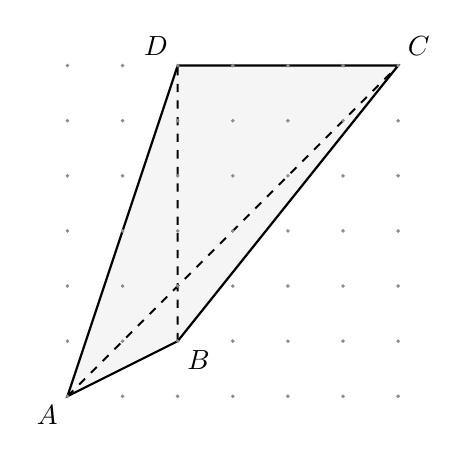
\begin{tikzpicture}[x=7mm,y=7mm]
\draw[fill=black!4,line width=.8pt] (0,0)--(2,1)--(6,6)--(2,6)--cycle;
\draw[dashed,line width=.7pt] (0,0)--(6,6) (2,1)--(2,6);
\foreach \x in {0,...,6}\foreach \y in {0,...,6}\fill[black!45] (\x,\y) circle[radius=.25mm];
\node[below left] at (0,0){$A$};\node[below right] at (2,1){$B$};
\node[above right] at (6,6){$C$};\node[above left] at (2,6){$D$};
\end{tikzpicture}\par\small Compact adult diagram; not a cutting template.
\end{minipage}\hfill
\begin{minipage}{.58\linewidth}
Example: $A=(0,0),B=(2,1),C=(6,6),D=(2,6)$.
\begin{tabular}{@{}lrrr@{}}\toprule
Region & $I$ & $B$ & $A$\\\midrule
$ABC$ & 0 & 8 & 3\\
$ACD$ & 7 & 12 & 12\\
$ABD$ & 2 & 8 & 5\\
$BCD$ & 6 & 10 & 10\\
$ABCD$ & 12 & 8 & 15\\\bottomrule
\end{tabular}\par
The two decompositions give $3+12=5+10=15$. The target triangle has an interior-to-the-bounding-rectangle vertex; its rectangle complement includes a quadrilateral. Three complementary right triangles are not a universal shortcut.
\end{minipage}
\end{center}

\subhead{5. Remove and reattach polygon ears}
A positive-area simple polygon can be triangulated by ears using its own vertices. Ignore redundant collinear corners in the triangulation description, but keep \emph{all} their dots in $B$. An ear is a triangle between two neighboring sides and an internal diagonal, whose removal leaves a smaller simple polygon. Induct on the number of vertices: all lattice triangles are proved; remove a nondegenerate ear, prove the smaller polygon, then reattach the ear along its one full lattice diagonal. That join satisfies the exact-side assumptions. Both $Q$ and area add, proving the original polygon. An arbitrary order of adjoining triangles need not be legal; ear removal/reattachment supplies the needed order.

\textbf{Adult proof support.} Offer a concrete axis-side example before the bridge, and a concave outline before the ear argument. Children may stop at a family they can explain. The bridge is an independently repaired argument for this packet; NRICH supports the overall additivity route, not this exact construction. Exhaustive tests of 2,148 small-grid triangles check its implementation; the geometric argument above proves the unrestricted statement.
\newpage

\heading{Problems 9--10 / student pp.\,9--10 / holes after the core}
\subhead{Problem 9: one hole, independent subtraction first}
The printed outer square is $(0,0),\allowbreak(4,0),\allowbreak(4,4),\allowbreak(0,4)$; hole corners are $(1,1),\allowbreak(3,1),\allowbreak(3,3),\allowbreak(1,3)$. \textbf{Area $16-4=12$, $I=0$, $B=16+8=24$}. Its central dot $(2,2)$ is removed; all eight surrounding hole-side dots are boundary. The uncorrected expression gives $0+12-1=11$, one too small. The one-hole rule is $A=I+B/2$.

A valid second test fits the actual $0\leq x\leq6$, $0\leq y\leq3$ board. Outer rectangle $(0,0),\allowbreak(6,0),\allowbreak(6,3),\allowbreak(0,3)$; unit-square hole $(1,1),\allowbreak(2,1),\allowbreak(2,2),\allowbreak(1,2)$. Independent area $18-1=17$. Filled outer counts are $I_o=10,B_o=18$; the hole has $I_h=0,B_h=4$. Thus region $I=6,B=22$, and $6+11=17$. A hole with no inside dot is still a hole.
\hints{Use a duplicate to measure the outer filled shape and the removed shape separately.}{Touch every inner-outline dot. Is it inside the remaining region, on its boundary, or removed?}{Compare the independently found area with the old expression. Does the same difference occur for your second hole?}
\textbf{If stuck.} Work with the printed ring only, keeping the old result and actual area side by side. Delay the new construction until separated-loop and removed-dot conventions are retained. One checked correction suggests a rule; the subtraction argument below proves it.

\subhead{Problem 10: a two-hole witness and any number of holes}
Use outer $(0,0),\allowbreak(6,0),\allowbreak(6,4),\allowbreak(0,4)$, with unit-square holes
\[(1,1),\allowbreak(2,1),\allowbreak(2,2),\allowbreak(1,2),\quad (4,1),\allowbreak(5,1),\allowbreak(5,2),\allowbreak(4,2).\]
Both holes lie strictly inside the $0\leq x,y\leq6$ board's outer shape and their closures are separate. The region remains connected. Independent area is $24-1-1=22$. The filled rectangle has $I_o=15,B_o=20$; removing the two holes' eight boundary dots leaves $I=7$, and $B=20+4+4=28$. Old expression: $7+14-1=20$; adding $h=2$ gives \textbf{22}.

\textbf{General proof by set subtraction.} Let the filled outer polygon have $I_o,B_o,A_o$, and each filled hole have $I_j,B_j,A_j$. Strict containment and pairwise disjoint closures give
\[I=I_o-\sum_{j=1}^{h}(I_j+B_j),\qquad B=B_o+\sum_{j=1}^{h}B_j,\qquad A=A_o-\sum_{j=1}^{h}A_j.\]
Each hole's inside \emph{and boundary} dots used to be inside the filled outer polygon. Its boundary dots now join $B$; its inside dots disappear from the region. Apply the already proved no-hole theorem to each filled polygon:
\begin{align*}
A&=I_o+B_o/2-1-\sum_j(I_j+B_j/2-1)\\
 &=\left[I_o-\sum_j(I_j+B_j)\right]+\tfrac12\left[B_o+\sum_jB_j\right]-1+h\\
 &=I+B/2-1+h.
\end{align*}
No dot is removed twice because the hole closures are disjoint. Nested loops defining islands, touching loops and disconnected shapes need different bookkeeping and are not claimed by this task's rule.
\hints{Make the outer shape first; on a duplicate remove two small, separated holes.}{Keep one record of the filled outer shape. Which dots leave its inside category with each hole?}{For each hole, distinguish its inside dots from its boundary dots. Can you account for the change in both counts?}
\textbf{If stuck.} Keep the two-hole experiment and its independent area. Save the $h$-hole proof for another visit; do not require a child to operate symbolic sums to participate in the construction.
\newpage

\heading{Sources, provenance and what to keep after the session}
\subhead{Mathematical and teaching precedents actually consulted}
\textbf{Laura Givental, Maria Nemirovskaya and Ilya Zakharevich, \emph{Math Circle by the Bay: Topics for Grades 1--5}} (AMS, 2018), printed pp.\,129--134, Problems 5.30--5.34 (local PDF pp.\,142--147). These pages supply the point-count investigation, independent area checks, formula limits and hole continuation. The source's printed p.\,129 reports that autonomous discovery was not expected; p.\,131 describes breaking long calculations into parts; p.\,134 distinguishes tested conjectures from proof and reports proof beyond those students' readiness. These are source observations. Our concrete routes, mark styles, hour estimates and readiness gates are \emph{untested local adaptations}, not claims that the source piloted this packet.

\textbf{Cambridge NRICH, \href{https://nrich.maths.org/problems/picks-theorem}{Pick's Theorem}}, Problem, Getting Started and Teachers' Resources: contrasting polygons and fixed-count comparisons. \textbf{\href{https://nrich.maths.org/problems/proof-picks-theorem}{Proof of Pick's Theorem}}, the additivity/rectangle/triangle route and final no-holes note: overall proof structure. Local downloaded versions were consulted. Their age labels are 14--16 and 16--18; these labels do not establish elementary fit. The two-diagonal general-triangle bridge and explicit legal-join/ear order in this guide are our independently repaired proof, not that exact argument attributed to NRICH.

\textbf{Natasha Rozhkovskaya, \emph{Math Circles for Elementary School Students: Berkeley 2009 and Manhattan 2011}} (AMS, 2014), Lesson 3, ``At the lesson,'' item 1, and Lesson 8, ``At the lesson,'' item 2 (local EPUB \nolinkurl{OEBPS/part0013.xhtml} and \nolinkurl{part0018.xhtml}). The first gives children time to attempt a problem before the teacher organizes it visibly; the second reports unequal writing speeds and reduced copying. These source observations support, by our inference, child attempts before pooled records and one recoverable shape rather than several simultaneous tallies.

\textbf{Organizer evidence.} First-year \emph{Handouts 1.docx}, tiled figurate squares/triangular scaling, and \emph{Handouts 4.docx}, Problems 4.2--4.5, give concrete tiling precedents. README/context report success with physical pattern blocks and difficulty retaining paper lamp rules. This supports visible state and partner checking; it does not establish prior knowledge of halves or Pick. Fixed tables and staffing come from the current October 3 context.

Wording, page composition, compact proof figure, preparation calculations, witnesses and verification scripts were authored for this guide around established mathematics. The rectangle/parallelogram/L-shape/ring data come from the checked new outline and final student figures; novelty of the mathematics is not claimed. Portable guide source contains only authored TeX, builder, verifier and README. It bundles no third-party books, downloaded pages or borrowed workflow exemplars. Root \nolinkurl{REPUBLISHING.md} was read and preserved; attribution is not publication clearance. This guide accompanies student version \textbf{N57-S-final-v2}; no remote version was written or checked.

\subhead{Record actual use, evidence and a next question}
For each fixed table, record the date, people present, problems actually reached, constructions retained, and the next starting point. Keep one child's marked drawing or exact words. Label a claim \emph{tried}, \emph{conjectured}, \emph{checked in named cases}, or \emph{explained for a stated family}. Note whether adults read/recorded, helped handle tools, or had to make the mathematical choices. Separate observations from hypotheses about causes or grade readiness.

Track this lattice-area theme across distinct visits: independent area/count comparisons; area-6 inverse constructions; seams; triangle/polygon proof; holes. Week 31's bonus already uses empty triangles and its guide mentions Pick; Week 48 uses cell-cover bounds. This visit adds full area/inside/boundary relationships and legal seam cancellation. File presence is not evidence a returning child used those earlier investigations. Save incomplete work for a genuine continuation rather than repeat the same catalog.

\textbf{Verification and status.} Every stated count/witness and geometric area was recomputed by the portable verifier, including both seam cases and the repaired proof bridge. All ten guide pages were rendered and visually inspected; copied-source and ZIP-extracted builds matched in text, Letter dimensions and every 144-dpi rendered pixel. These are digital checks. Physical rehearsal and classroom piloting remain \textbf{unperformed}; record their results before treating the route or material quantities as classroom-tested.
\end{document}
